\begin{itemize}
  \item Background on Coverage
  \item Limitations of current concurrency coverage criterias
  \item what it takes to define a good coverage metric
  \begin{itemize}
    \item thorough observation of target bugs, their symptoms, their causes and fixes.
    \item according to \cite{}
  \end{itemize}
  \item
\end{itemize}

\subsection{Coverage Idea}
Existing concurrent coverage metrics target either synchronization primitives or memory access for Java. In Java, locks and other serialization techniques like conditional variables and semaphores usually provide mutual exclusion and memory protection (i.e., no “direct” communication between threads are involved. In Go, a goroutine can directly unblock another goroutine)
\\
-	For example in Java,  thread A either is blocked from entering a critical section (or mutually exclusive section) protected by lock L or is blocking other threads (e.g., thread B) from entering the critical section.
\\
If, during testing (e.g., exploring schedule-space and interleavings), one thread never gets blocked and always blocks other goroutines on a lock operation, it is often the case that there is a possible untested and important interleaving. Blocked/blocking coverage model is the basis of existing synchronization coverages. A 100\% coverage on operation e is achieived when each thread t\_i performs e in blocked and blocking way, at least one each.
-	Test coverage analysis: defining a set of tasks and check that each task is covered in testing phase. A coverage metric is defined based on the tasks to measure quality and completeness of testing.
-	Superior coverage metrics like source-line coverage and branch coverage are popular because they have four major characteristics:
\begin{itemize}
  \item The metric should be well-understood by the developer or tester. Models to run tasks for measuring metrics should construct statically by instrumenting the source-code.
  \item All tasks should be coverable. For a few that are not (due to technical limitations or program semantics), a review process is required.
  \item Every uncovered task should yield an action: add more tests or remove dead code (re-design)
  \item Some action should be taken upon reaching a threshold of coverage(e.g., testing phase termination when reaching 100\% statement coverage)
\end{itemize}

-	In addition to blocked/blocking, other synchronization coverage metrics like sync-pair, follows, PSet, HaPSet are defined to measure quality of interleaving-space testing of concurrent software, mostly in Java and C++.
\\
-	Another important factor is the importance of common bug scenarios based on the platform specification and target class of bugs. Coverage metrics that are defined for races or atomicity-violation in Java are not applicable for blocking bugs (non-memory-access bugs) in Go. Hence, new coverage metrics are required.

\subsection{New coverage models}
Based on my observations from studying GoKer bugs using the GOAT infrastructure, here is my proposal for a set of coverage models to measure the quality of interleaving-space search of GOAT random and bounded schedule permutation:
\begin{itemize}
  \item The Select-case statement is the major cause of rare bugs specific to Go. Multiple blocking actions (send/recv) might get blocked on a select statement. Once one or more becomes available, Go picks one “randomly”. A default case make select “unblocking”. When no blocking case is available, the default case let the goroutine to make progress. GOAT and ECT are capable of identifying the select statement behavior (e.g., which case have been selected in each execution of select).
  \item Unlike lock operations that might be blocked  or blocking, channel sends and receives are blocked or “unblocking”. Channel sends (receives) blocks a goroutine if the receiver (sender) is not ready or unblocks a goroutine if the receiver (sender) is already waiting. A channel send/recv might also be of type no-op (for buffered channels).

\end{itemize}

-	While existing synchronization coverages often ignore unlocks, I think unlocks are also important because they might (or might not) “unblock” a waiting goroutine (unblocking/no-op)
\stcmt{Why I think this is good?}
- It exploits the enhancement I made for Go tracer.
- The proposed coverage model idea is strong because:
- It follows the four rule of popular coverage metrics
- It is based on a thorough study of GoKer bugs
- I can generate a interesting tables to show the impact of the random scheduler-perturbations.
- It is novel and adds some scientific aspect to my thesis.

\subsection{Implementation}
It is crucial to maintain a static model of goroutines and coverage metrics during testing executions. I obtain such model in two ways:
-	Statically: The concurrency usage (ie, source line numbers that perform actions go/send/recv/lock/unlock/wait/done/sig/bcast/select) is obtained from traversing the source AST. Such concurrency usage model has two purposes:
- Critical points to inject sched\_yield before them.
- A pre-execution model of testing tasks. During testing phase, we map each source line with its corresponding action to an event in ECT based on its call-stack.
-	Dynamically: A good test run is required to obtain some models dynamically. (I will explain GGTree and stack later. Why do we need GGTree?)




\begin{figure}
\centering
  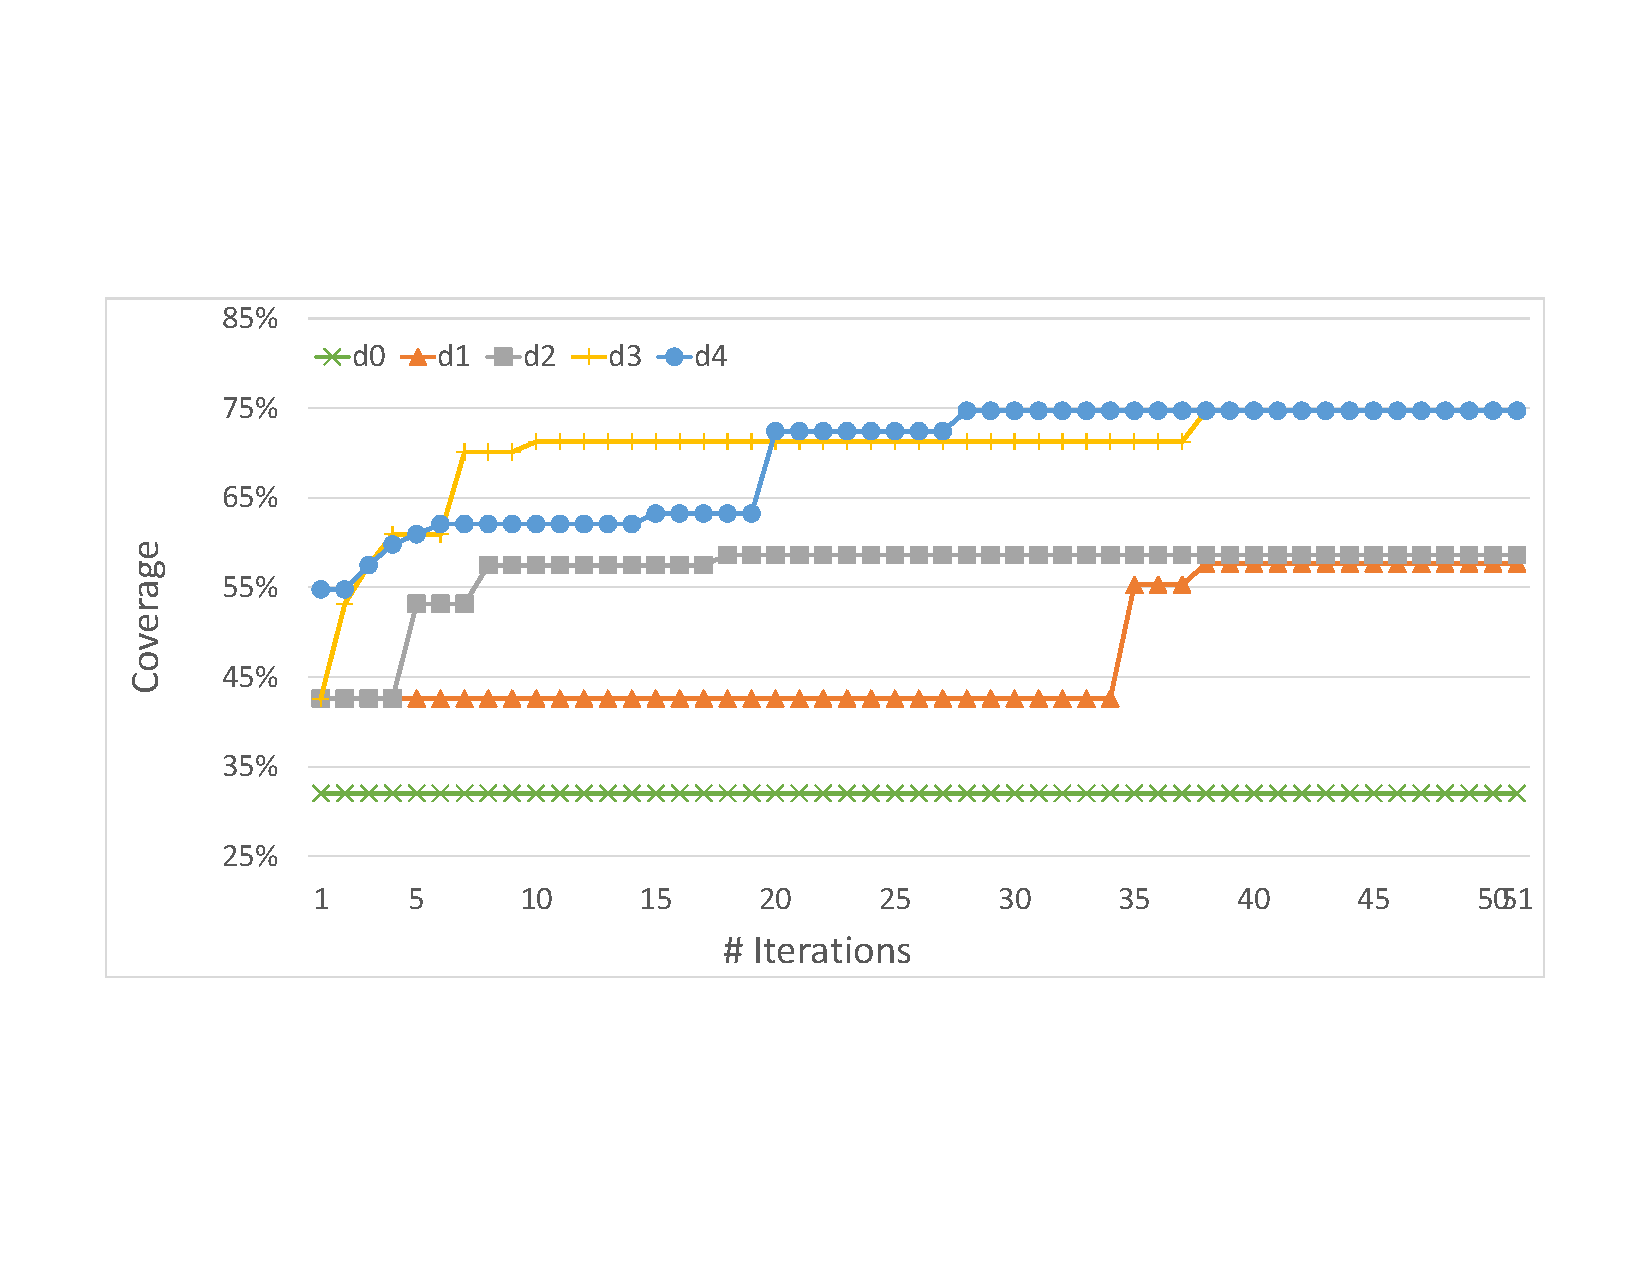
\includegraphics[width=.95\linewidth]{figs/coverage_etcd7443.pdf}
  \caption{etcd7442 coverage}
  \label{fig:etcd_coverage}
\end{figure}


\begin{figure}
\centering
  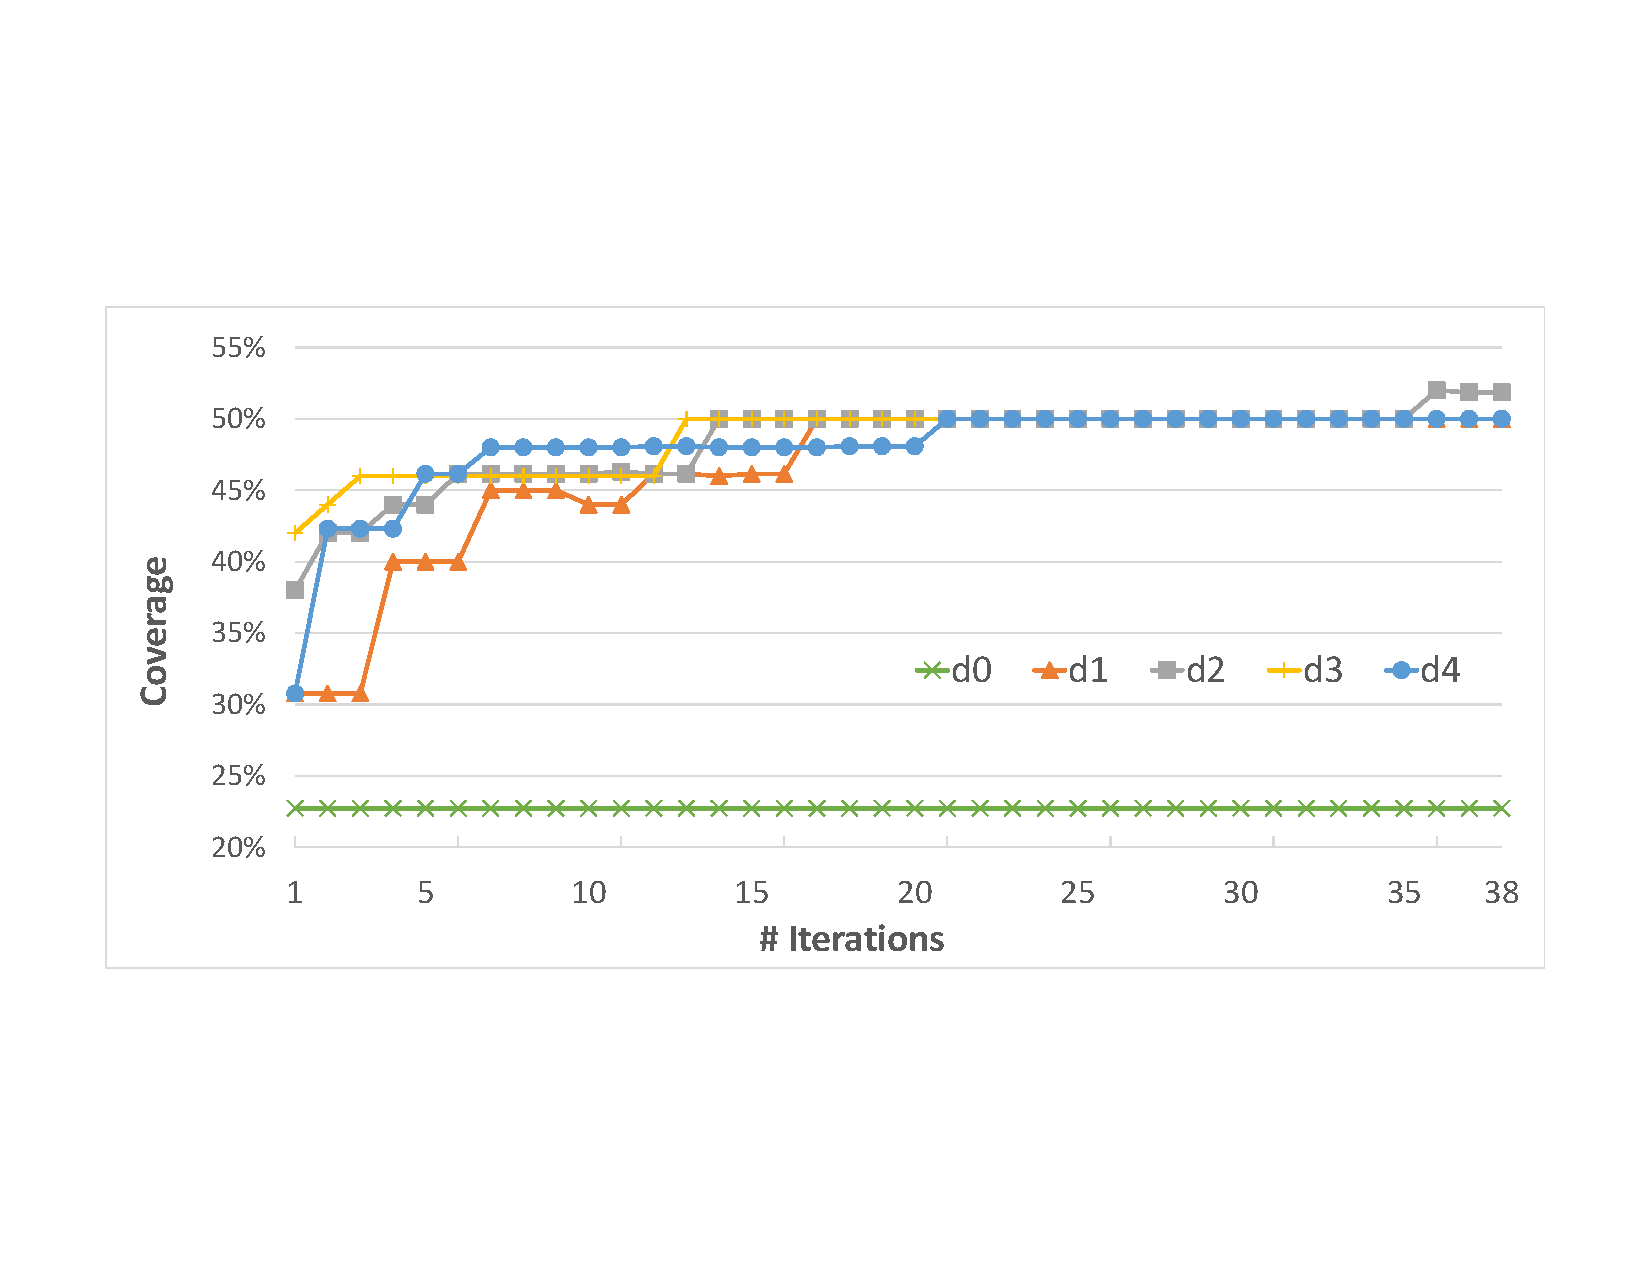
\includegraphics[width=.95\linewidth]{figs/coverage_kubernetes11298.pdf}
  \caption{kuberenetes11298 coverage}
  \label{fig:kubernetes_coverage}
\end{figure}
